% Generated by code/needham.py -- do not edit by hand.
\definecolor{qocA}{rgb}{0.00,0.45,0.70}
\definecolor{qocB}{rgb}{0.90,0.60,0.00}
\definecolor{qocC}{rgb}{0.00,0.62,0.45}
\definecolor{qocD}{rgb}{0.80,0.40,0.00}
\definecolor{qocE}{rgb}{0.80,0.60,0.70}
\definecolor{qocF}{rgb}{0.35,0.70,0.90}
\begin{tikzpicture}[ink/.style={line width=0.9pt, ndInk}, faint/.style={line width=0.4pt, ndInk!35}, dashedink/.style={line width=0.5pt, ndInk!55, dash pattern=on 2.5pt off 2pt}, vec/.style={->, >=stealth, line width=1.2pt}, note/.style={font=\footnotesize\itshape, text=ndInk!85, align=center}, pointer/.style={->, >=stealth, line width=0.4pt, ndInk!60, shorten >=2pt, shorten <=1pt}, dot/.style={circle, fill=ndInk, inner sep=0pt, minimum size=3.4pt}, wash/.style={fill=ndSky, fill opacity=0.55}, every node/.style={text=ndInk}]
\definecolor{ndInk}{rgb}{0.13,0.13,0.18}
\definecolor{ndPaper}{rgb}{0.99,0.96,0.88}
\definecolor{ndSky}{rgb}{0.84,0.91,0.98}
\definecolor{ndRose}{rgb}{0.98,0.86,0.84}
\definecolor{ndBlue}{rgb}{0.13,0.36,0.66}
\definecolor{ndRed}{rgb}{0.78,0.20,0.16}
\definecolor{ndGold}{rgb}{0.88,0.62,0.10}
\definecolor{ndGreen}{rgb}{0.18,0.52,0.30}
\fill[ndRose, fill opacity=0.75] (0.000,0.000) -- (2.511,-0.252) -- (1.592,1.550) -- cycle;
\fill[ndRose, fill opacity=0.75] (3.184,3.099) -- (1.592,1.550) -- (3.184,0.689) -- (4.104,1.298) -- cycle;
\fill[ndRose, fill opacity=0.75] (2.511,-0.252) -- (5.023,-0.504) -- (4.104,1.298) -- cycle;
\fill[ndSky, fill opacity=0.85] (2.511,-0.252) -- (4.104,0.092) -- (4.104,1.298) -- (1.592,1.550) -- (1.592,0.344) -- cycle;
\draw[line width=1.0pt, ndBlue] (2.511,-0.252) -- (4.104,0.092);
\draw[line width=1.0pt, ndBlue] (2.511,-0.252) -- (4.104,1.298);
\draw[line width=1.0pt, ndBlue] (2.511,-0.252) -- (1.592,1.550);
\draw[line width=1.0pt, ndBlue] (2.511,-0.252) -- (1.592,0.344);
\draw[line width=1.0pt, ndBlue] (4.104,0.092) -- (4.104,1.298);
\draw[line width=0.5pt, ndBlue!70, densely dashed] (4.104,0.092) -- (3.184,0.689);
\draw[line width=1.0pt, ndBlue] (4.104,1.298) -- (1.592,1.550);
\draw[line width=0.5pt, ndBlue!70, densely dashed] (4.104,1.298) -- (3.184,0.689);
\draw[line width=1.0pt, ndBlue] (1.592,1.550) -- (1.592,0.344);
\draw[line width=0.5pt, ndBlue!70, densely dashed] (1.592,1.550) -- (3.184,0.689);
\draw[line width=0.5pt, ndBlue!70, densely dashed] (1.592,0.344) -- (3.184,0.689);
\draw[ink] (0.000,0.000) -- (5.023,-0.504);
\draw[dashedink] (0.000,0.000) -- (3.184,0.689);
\draw[ink] (0.000,0.000) -- (3.184,3.099);
\draw[dashedink] (5.023,-0.504) -- (3.184,0.689);
\draw[ink] (5.023,-0.504) -- (3.184,3.099);
\draw[dashedink] (3.184,0.689) -- (3.184,3.099);
\draw[line width=1.6pt, ndBlue!45] (0.000,0.000) -- (2.511,-0.252);
\node[dot, fill=ndInk, minimum size=3.2pt] at (0.000,0.000) {};
\node[dot, fill=ndInk, minimum size=3.2pt] at (5.023,-0.504) {};
\node[dot, fill=ndBlue, minimum size=3.2pt] at (3.184,0.689) {};
\node[dot, fill=ndInk, minimum size=3.2pt] at (3.184,3.099) {};
\node[dot, fill=ndBlue, minimum size=3.2pt] at (2.511,-0.252) {};
\node[dot, fill=ndBlue, minimum size=3.2pt] at (4.104,0.092) {};
\node[dot, fill=ndBlue, minimum size=3.2pt] at (4.104,1.298) {};
\node[dot, fill=ndBlue, minimum size=3.2pt] at (1.592,1.550) {};
\node[dot, fill=ndBlue, minimum size=3.2pt] at (1.592,0.344) {};
\node[font=\scriptsize, anchor=east] at (-0.100,0.000) {$O$};
\node[font=\scriptsize, anchor=west] at (5.123,-0.504) {$A_1$};
\node[font=\scriptsize, anchor=south] at (3.184,3.199) {$A_3$};
\node[font=\scriptsize, anchor=north] at (2.511,-0.372) {$L:\ \mathrm{CNOT}$};
\node[font=\scriptsize, anchor=south east] at (1.472,1.600) {$P:\ \sqrt{\mathrm{SWAP}}$};
\node[font=\scriptsize, anchor=west] at (4.224,1.348) {$N:\ \sqrt{\mathrm{SWAP}}^{\,\dagger}$};
\node[font=\scriptsize, anchor=east] (lQ) at (-0.60,1.05) {$Q:\ \sqrt{\mathrm{iSWAP}}$};
\draw[pointer] (lQ.east) to[bend left=10] (1.652,0.344);
\node[font=\scriptsize, anchor=west] (lA2) at (6.35,0.80) {$A_2:\ \mathrm{iSWAP}$};
\draw[pointer] (lA2.west) to[bend right=10] (3.124,0.689);
\node[font=\scriptsize, anchor=west] (lM) at (6.35,0.15) {$M$};
\draw[pointer] (lM.west) to[bend right=10] (4.044,0.092);
\node[circle, draw=ndRed, fill=white, line width=0.8pt, inner sep=0pt, minimum size=4pt] at (1.256,-0.126) {};
\node[font=\scriptsize\bfseries, text=ndRed, anchor=south] at (1.256,-0.066) {1};
\node[circle, draw=ndRed, fill=white, line width=0.8pt, inner sep=0pt, minimum size=4pt] at (2.848,0.218) {};
\node[font=\scriptsize\bfseries, text=ndRed, anchor=south] at (2.848,0.278) {3};
\node[font=\scriptsize\bfseries, text=ndRed, anchor=south east] at (2.411,-0.232) {2};
\node[note, anchor=south west, text=ndBlue] (pe) at (3.684,2.749) {perfect entanglers:\\ half the chamber,\\ $\pi^3/48$ of $\pi^3/24$};
\draw[pointer] (pe.south west) to[bend right=15] (3.098,0.870);
\node[note, anchor=north, text=ndRed!80!ndInk] (nc) at (5.423,-0.954) {not perfect entanglers:\\ the three corners};
\draw[pointer] (nc.north) to[bend right=10] (3.985,0.138);
\node[note, anchor=north, text=ndBlue] (cu) at (0.102,-0.600) {of the controlled-$U$ gates\\ only CNOT};
\draw[pointer] (cu.north) -- (0.628,-0.123);
\node[font=\small, anchor=north] at (2.511,-1.954) {(a) the perfect entanglers in the Weyl chamber};
\draw[faint] (9.500,2.150) circle (0.720);
\draw[faint] (8.660,2.150) -- (10.340,2.150);
\draw[faint] (9.500,1.310) -- (9.500,2.990);
\draw[line width=1.2pt, ndRed] (10.009,1.641) -- (10.009,2.659);
\node[dot, fill=ndBlue, minimum size=3.2pt] at (10.009,1.641) {};
\node[font=\tiny, text=ndInk!80, anchor=west] at (10.099,1.641) {$\times2$};
\node[dot, fill=ndBlue, minimum size=3.2pt] at (10.009,2.659) {};
\node[font=\tiny, text=ndInk!80, anchor=west] at (10.099,2.659) {$\times2$};
\draw[ndRed, line width=0.7pt] (9.440,2.090) -- (9.560,2.210) (9.440,2.210) -- (9.560,2.090);
\node[font=\scriptsize\bfseries, text=ndRed] at (8.730,2.920) {1};
\node[font=\scriptsize] at (9.500,3.190) {$[\tfrac\pi4,0,0]$};
\node[note, anchor=north] at (9.500,1.250) {$0$ outside:\\ not a perfect\\ entangler};
\draw[faint] (11.750,2.150) circle (0.720);
\draw[faint] (10.910,2.150) -- (12.590,2.150);
\draw[faint] (11.750,1.310) -- (11.750,2.990);
\draw[line width=1.2pt, ndBlue] (11.750,1.430) -- (11.750,2.870);
\node[dot, fill=ndBlue, minimum size=3.2pt] at (11.750,1.430) {};
\node[font=\tiny, text=ndInk!80, anchor=west] at (11.840,1.430) {$\times2$};
\node[dot, fill=ndBlue, minimum size=3.2pt] at (11.750,2.870) {};
\node[font=\tiny, text=ndInk!80, anchor=west] at (11.840,2.870) {$\times2$};
\draw[ndRed, line width=0.7pt] (11.690,2.090) -- (11.810,2.210) (11.690,2.210) -- (11.810,2.090);
\node[font=\scriptsize\bfseries, text=ndRed] at (10.980,2.920) {2};
\node[font=\scriptsize] at (11.750,3.190) {$[\tfrac\pi2,0,0]$};
\node[note, anchor=north] at (11.750,1.250) {$0$ on the hull:\\ CNOT, a perfect\\ entangler};
\draw[faint] (14.000,2.150) circle (0.720);
\draw[faint] (13.160,2.150) -- (14.840,2.150);
\draw[faint] (14.000,1.310) -- (14.000,2.990);
\filldraw[fill=ndSky, draw=ndBlue, line width=0.8pt] (13.491,1.641) -- (14.509,1.641) -- (14.509,2.659) -- (13.491,2.659) -- cycle;
\node[dot, fill=ndBlue, minimum size=3.2pt] at (13.491,1.641) {};
\node[dot, fill=ndBlue, minimum size=3.2pt] at (14.509,1.641) {};
\node[dot, fill=ndBlue, minimum size=3.2pt] at (14.509,2.659) {};
\node[dot, fill=ndBlue, minimum size=3.2pt] at (13.491,2.659) {};
\draw[ndRed, line width=0.7pt] (13.940,2.090) -- (14.060,2.210) (13.940,2.210) -- (14.060,2.090);
\node[font=\scriptsize\bfseries, text=ndRed] at (13.230,2.920) {3};
\node[font=\scriptsize] at (14.000,3.190) {$[\tfrac\pi2,\tfrac\pi4,0]$};
\node[note, anchor=north] at (14.000,1.250) {$0$ inside:\\ a perfect\\ entangler};
\node[font=\small, anchor=north, align=center] at (11.750,0.180) {(b) the eigenvalues of $m(U)$ and their convex hull};
\fill[ndSky] (8.900,-1.200) rectangle (11.750,-0.900);
\fill[ndRose] (11.750,-1.200) rectangle (14.600,-0.900);
\draw[ndInk!60, line width=0.4pt] (8.900,-1.200) rectangle (14.600,-0.900);
\node[font=\scriptsize, anchor=south west] at (8.850,-0.900) {by volume in the chamber};
\node[font=\scriptsize\bfseries, text=ndBlue, anchor=east] at (11.690,-1.050) {$50\%$};
\fill[ndSky] (8.900,-2.000) rectangle (13.753,-1.700);
\fill[ndRose] (13.753,-2.000) rectangle (14.600,-1.700);
\draw[ndInk!60, line width=0.4pt] (8.900,-2.000) rectangle (14.600,-1.700);
\node[font=\scriptsize, anchor=south west] at (8.850,-1.700) {by the Haar measure};
\node[font=\scriptsize\bfseries, text=ndBlue, anchor=east] at (13.693,-1.850) {$85\%$};
\node[font=\small, anchor=north, align=center] at (11.750,-2.150) {(c) the share of perfect entanglers};
\end{tikzpicture}
